\section{Emerging Trends and Future Directions}

In the rapidly evolving landscape of text-to-3D model generation, the previously discussed methods represent only a fraction of the innovative approaches currently shaping the field. These methods, each with their unique features and methodologies, contribute to the broader spectrum of advances in 3D model generation. However, more recent developments, such as Luma-AI's Genie method \citep{LumaAIGenie2023}, are pushing the boundaries further and overcoming many of the challenges faced by previous models.

Luma-AI's Genie, similar to the user-friendly approach of Midjourney \citep{Midjourney2023}, offers an accessible platform for 3D model generation. This service, operational on a Discord server \citep{discord}, allows users to input text descriptions. Upon receiving such input, Genie generates four preliminary models of the specified object. Users are then given the opportunity to refine each result. This iterative process, which typically takes around 10 minutes, culminates in the creation of a high-quality 3D representation. Notably, the use of Genie does not necessitate high-end hardware or additional platforms like Google Colab, as Luma AI manages the necessary computational aspects in the background. The model was published in November 2023 as a research preview to facilitate the creation of 3D models. However, no comprehensive details of how it works have yet been published.

The results achieved with Luma AI's Genie method are an example of the great progress made in this field. These advances demonstrate the potential of text-to-3D technologies for the fast and efficient creation of detailed, accurate 3D models. Some examples derived from this model are depicted in Figure~\ref{fig:GenieAI_robot} and Figure~\ref{fig:GenieAI_manta}. 

\begin{figure}[H]
    \centering
    \small
    \begin{subfigure}[b]{0.25\textwidth}
        \centering
        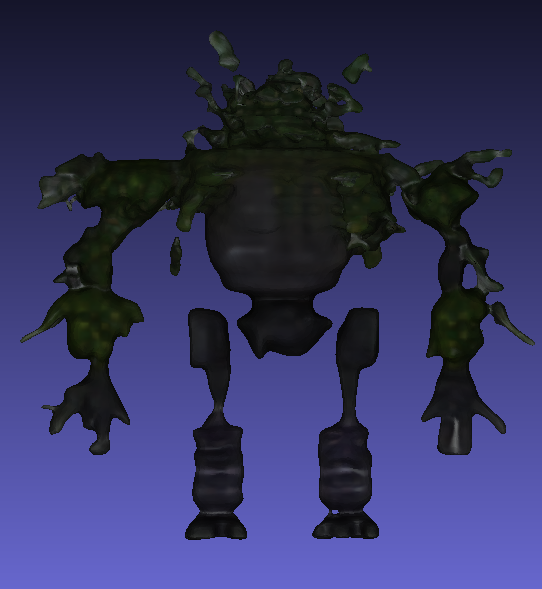
\includegraphics[width=\textwidth]{etc/Genie/plantRobot_coarse.png}
        \caption{}
    \end{subfigure}
    \begin{subfigure}[b]{0.26\textwidth}
        \centering
        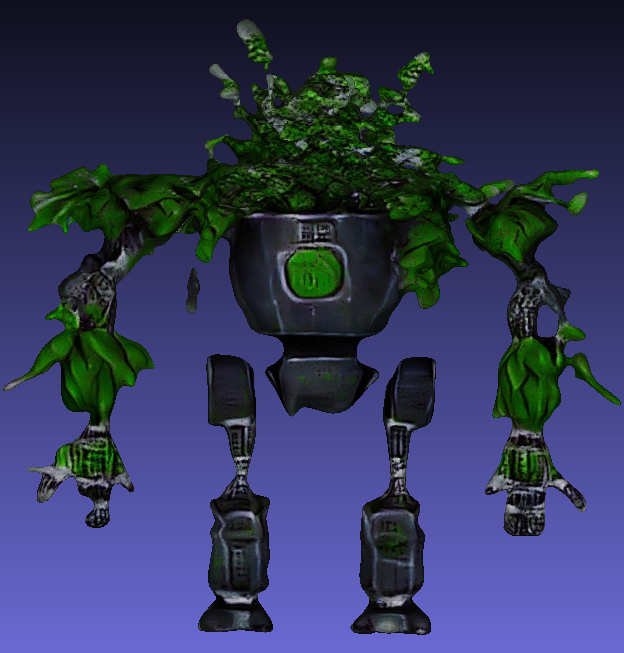
\includegraphics[width=\textwidth]{etc/Genie/plantRobot_fine_front.png}
        \caption{}
    \end{subfigure}
    \begin{subfigure}[b]{0.16\textwidth}
        \centering
        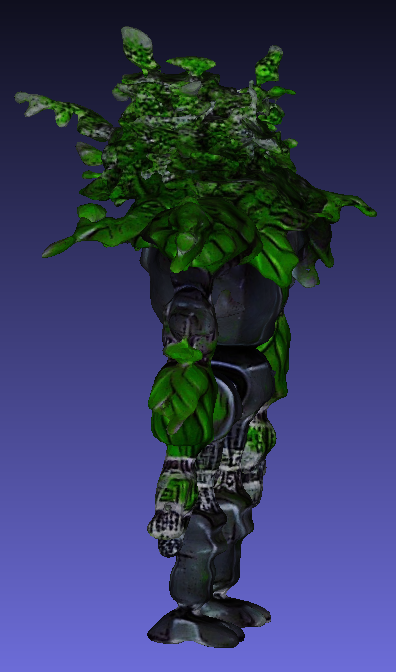
\includegraphics[width=\textwidth]{etc/Genie/plantRobot_fine_side.png}
        \caption{}
    \end{subfigure}
    \begin{subfigure}[b]{0.27\textwidth}
        \centering
        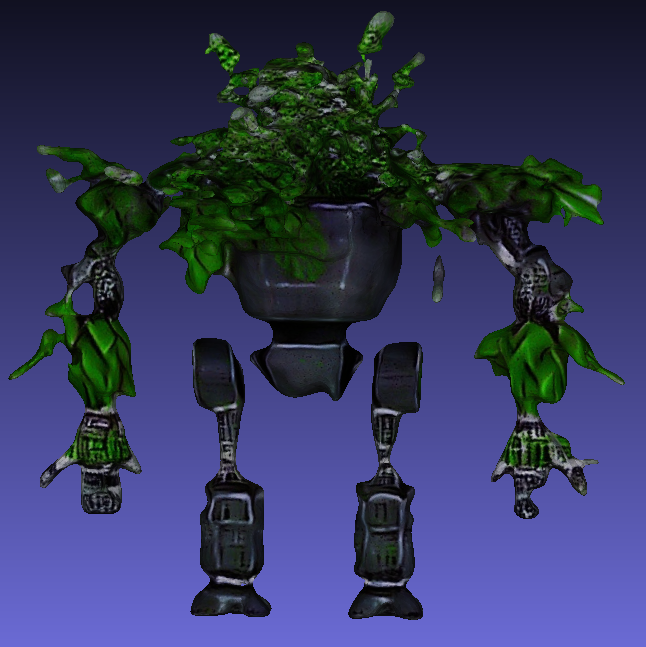
\includegraphics[width=\textwidth]{etc/Genie/plantRobot_fine_back.png}
        \caption{}
    \end{subfigure}
    \caption{The sequence shows the progressive refinement of a plant-based robot, beginning with a coarse initial model (a) and evolving to a high-quality representation with consistent detail across multiple views (b, c, d). The prompt used for generation was ``a robot made out of plants''.}~\label{fig:GenieAI_robot}
\end{figure}

\begin{figure}[H]
    \centering
    \small
    \begin{subfigure}[b]{0.23\textwidth}
        \centering
        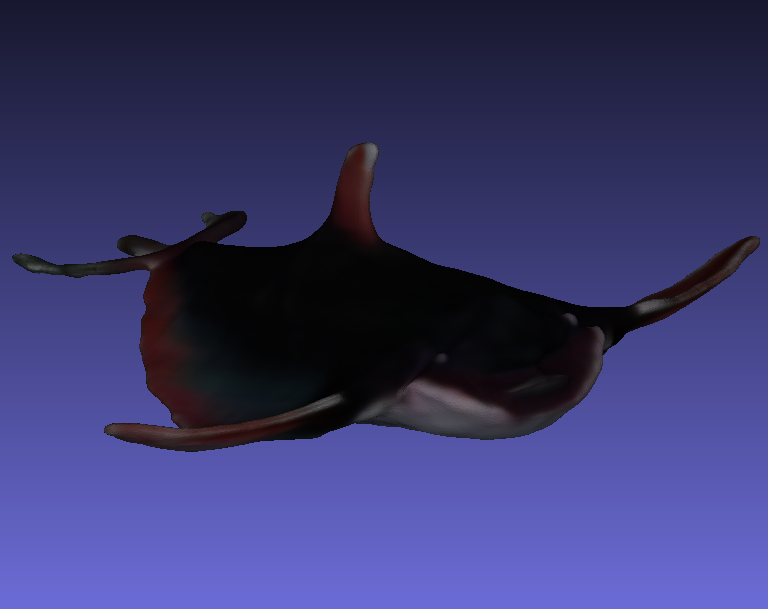
\includegraphics[width=\textwidth]{etc/Genie/manta_coarse_1.png}
        \caption{}
    \end{subfigure}
    \begin{subfigure}[b]{0.26\textwidth}
        \centering
        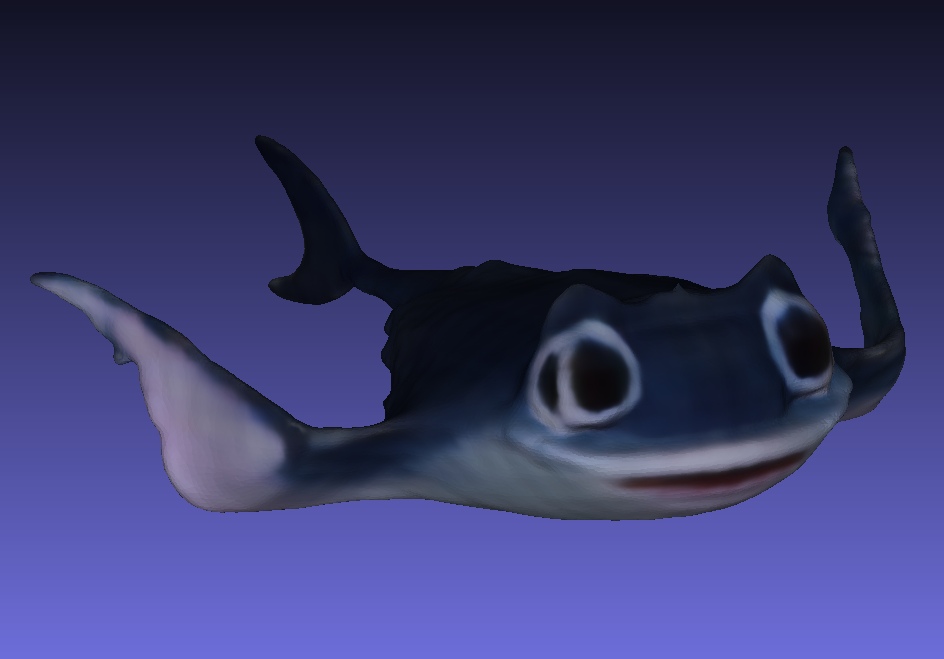
\includegraphics[width=\textwidth]{etc/Genie/manta_coarse_2.png}
        \caption{}
    \end{subfigure}
    \begin{subfigure}[b]{0.1825\textwidth}
        \centering
        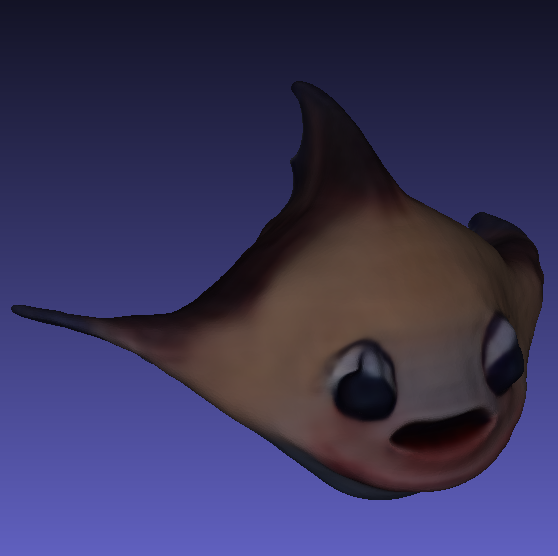
\includegraphics[width=\textwidth]{etc/Genie/manta_coarse_3.png}
        \caption{}
    \end{subfigure}
    \begin{subfigure}[b]{0.25\textwidth}
        \centering
        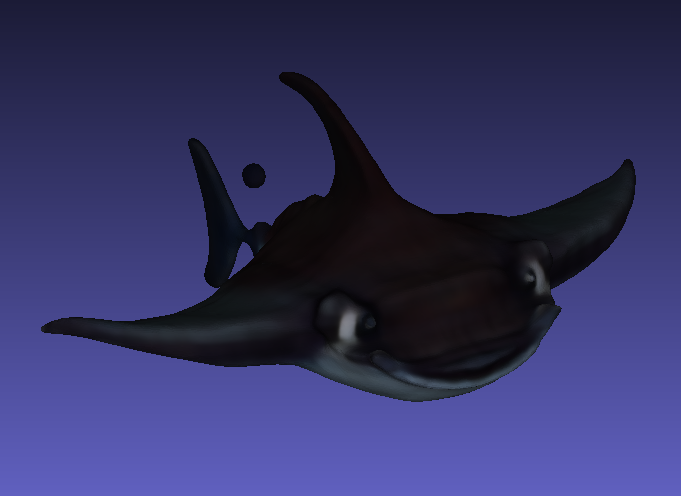
\includegraphics[width=\textwidth]{etc/Genie/manta_coarse_4.png}
        \caption{}
    \end{subfigure}

    \begin{subfigure}[b]{0.5\textwidth}
        \centering
        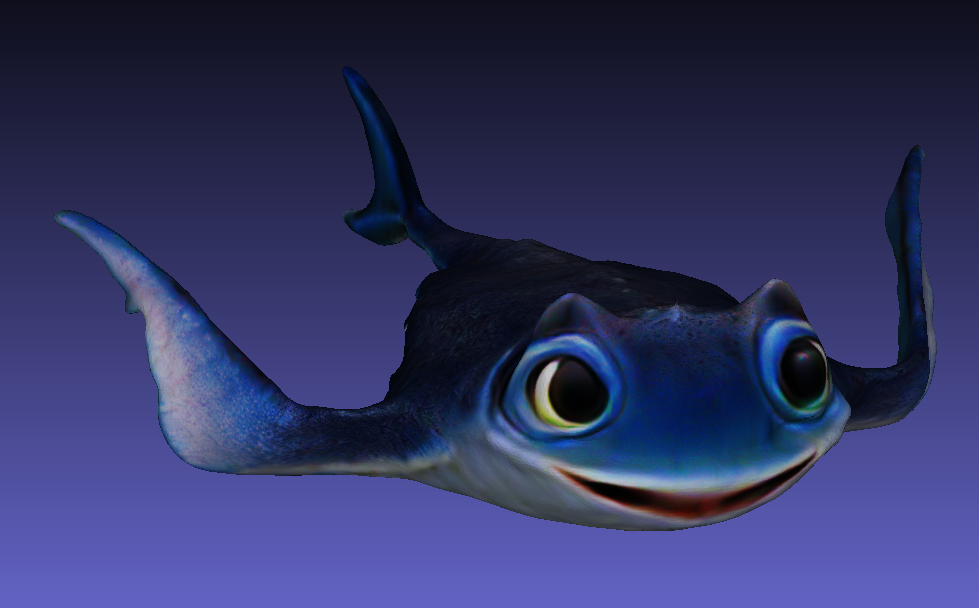
\includegraphics[width=\textwidth]{etc/Genie/manta_refine_2.png}
        \caption{}
    \end{subfigure}
    \begin{subfigure}[b]{0.42\textwidth}
        \centering
        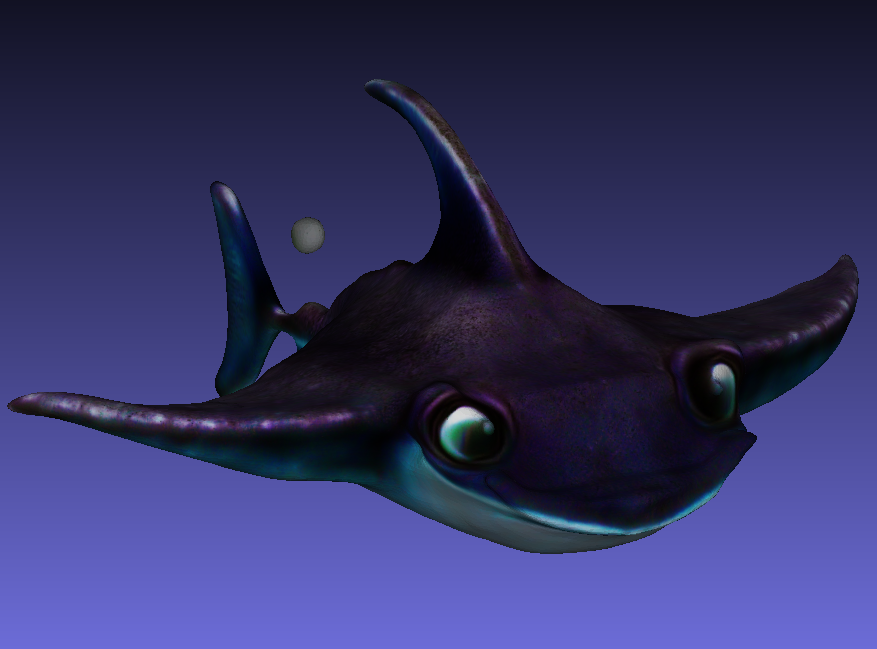
\includegraphics[width=\textwidth]{etc/Genie/manta_refine_4.png}
        \caption{}
    \end{subfigure}
    \caption{Parts (a-d) display the initial coarse models produced from the text prompt, while parts (e) and (f) showcase selected refined outcomes. The utilized prompt was ``A cute manta ray, Pixar style, high detail texture, 4K''.}~\label{fig:GenieAI_manta}

\end{figure}


Beyond 3D meshes or individual objects, the field of automatic 3D generation is also expanding to the conversion of video to 3D, opening up a new dimension of realistic scene creation. The latest research in this area uses Gaussian splatting \citep{kerbl3Dgaussians}, a technique characterized by remarkable results and reasonable hardware requirements. Gaussian splatting, a method for rendering radiation fields in real time, uses 3D Gaussians instead of traditional raster primitives such as triangles, enabling the creation of highly detailed and photorealistic scenes.

The pace of innovation in this field is rapid, as the timeline presented in Chapter~\ref{ch:models} of the thesis demonstrates. New methods and techniques come onto the market almost every month, offering promising results and new possibilities. This continuous development underlines the dynamism of automatic 3D model generation and points to an exciting future in which the boundaries of digital creativity and realism will be pushed further and further.
